\section{Mounted Filesystem and Matlab Integration}

Although StreamFS files and semantics are not POSIX compliant, we wrote a FUSE~\cite{fuse} imeplementation
that allows legacy applications to directly interact with StreamFS file and operate on them as if they were
locally mounted.

\begin{figure}[htb!]
\begin{center}
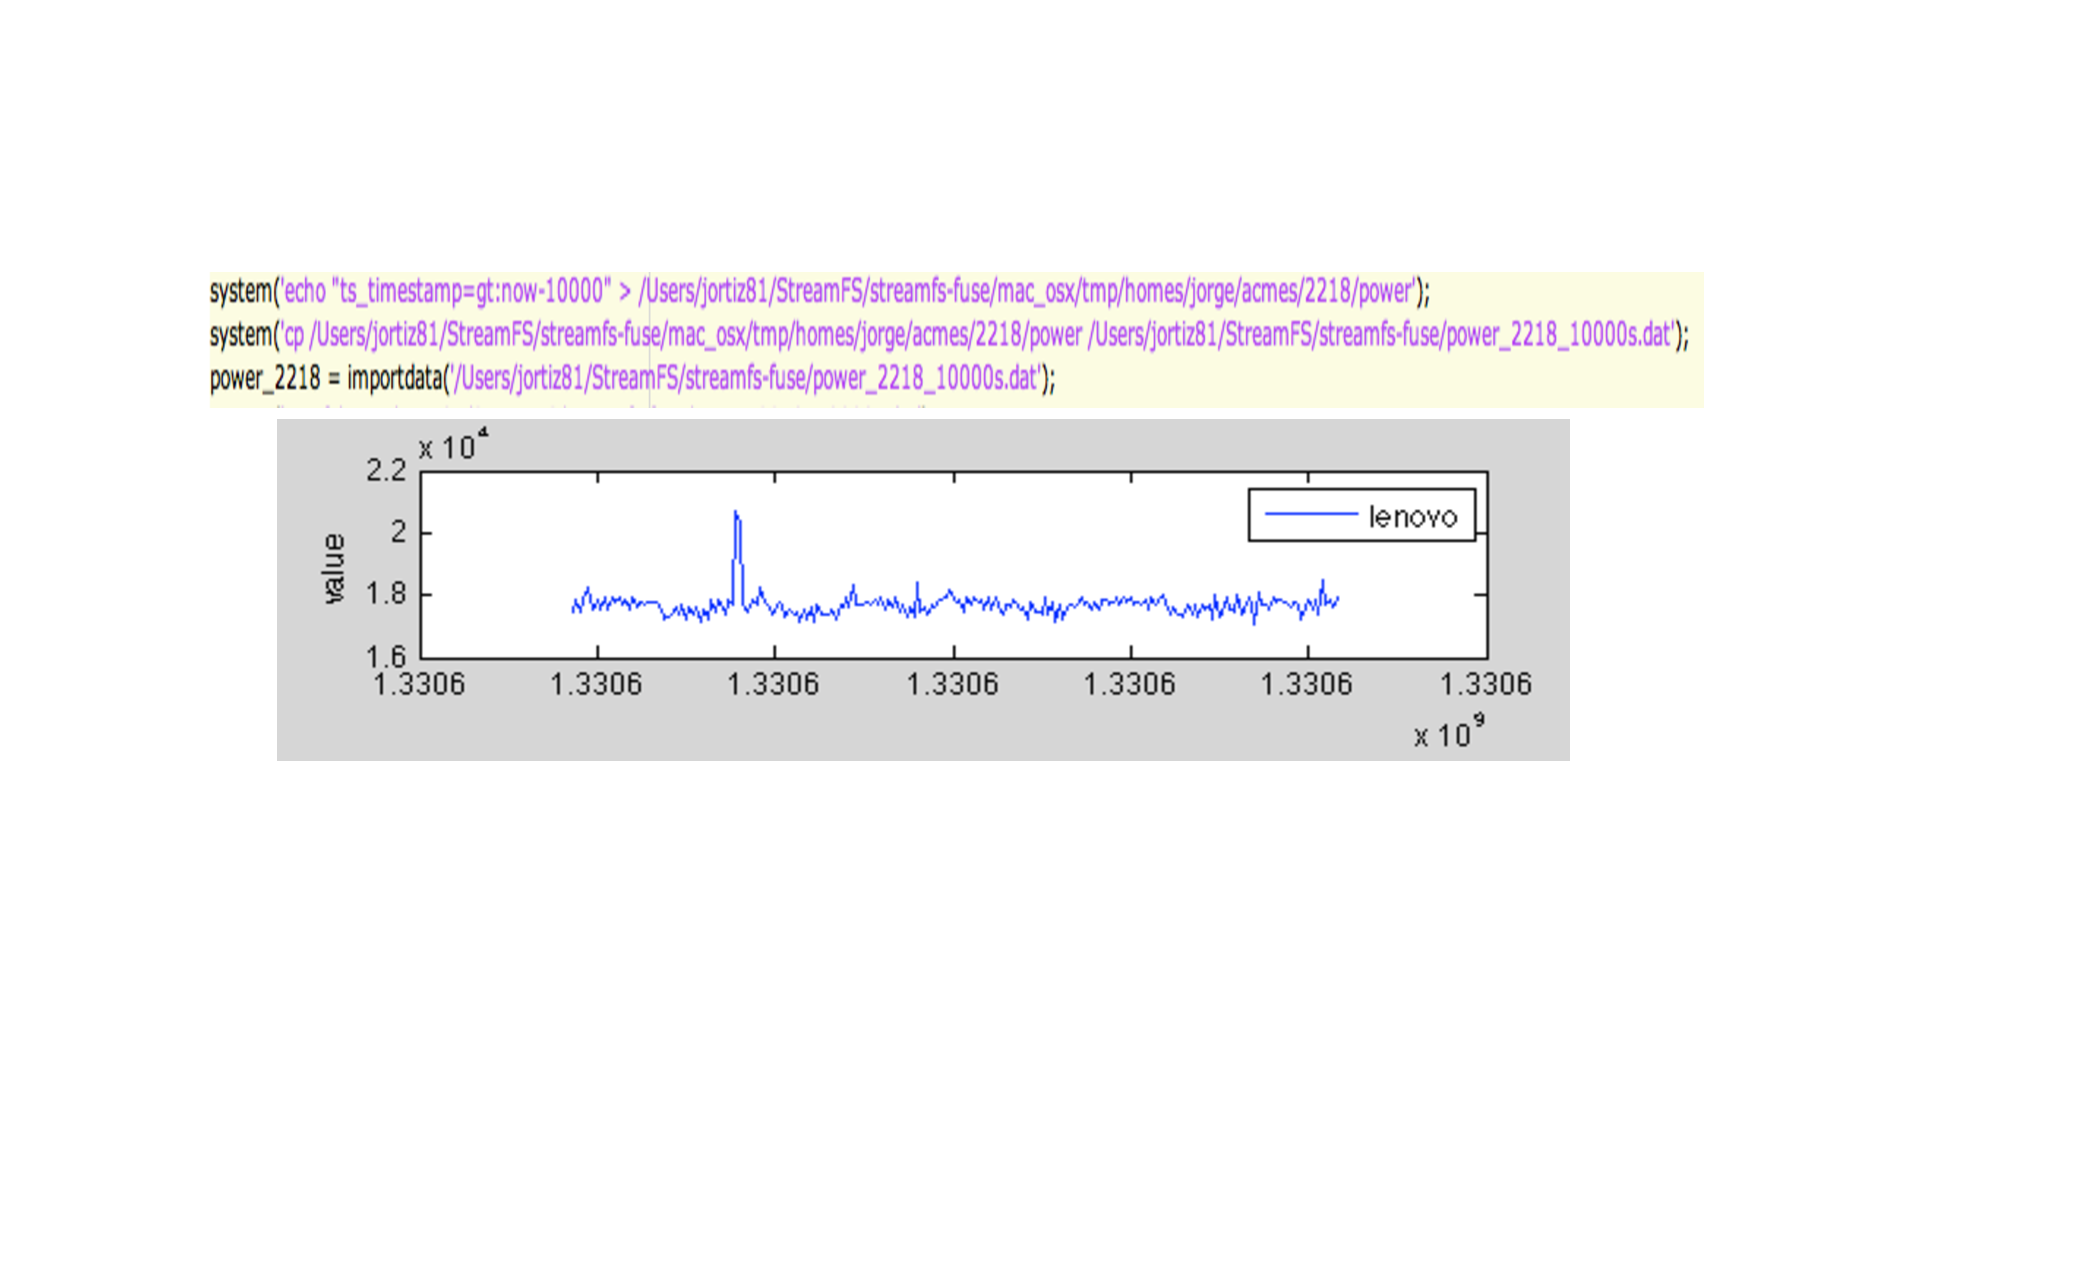
\includegraphics[scale=0.6]{figs/sfs_matlab}
\caption{SFSFuse implementation.  By mapping access and operational semantics to POSIX file operations
we enable legacy, desktop application to interact with the deployment directly.}
\label{fig:sfsfuse}
\end{center}
\end{figure}

Figure~\ref{fig:sfsfuse} shows a screen shot of mlatba reading and writing to local files that communicate 
with the StreamFS server.  This implementation represents an exercise and proof-point that the file abstract
can serve as a conveninient interface representing building deployments.  Although not an exact
fit, the semantics of StreamFS can be translated to make them look like a regular unix-style file.
Moreover, the security semantics are the same, since those are adopted directly.

\begin{table}[h]
\begin{center}
\begin{tabular}{| r | l |}
	\hline
	\textbf{operations} & \textbf{description} \\ \hline
	stream file read & Read the data from a timeseries query.    \\ \hline

	stream file write & Only accept query parameters. \\ hline

	container read & Folder read semantics.    \\ \hline

	container write & Folder write semantics.  \\ \hline

	tail -f & starts a stream subscription, writes to file \\ \hline

	pipe & writes file contents to pipe \\ \hline
\end{tabular}
\caption{Overview of StreamFS file-related API calls.  Library written in Java, PHP, and C.}
\label{tab:fuseops}
\end{center}
\end{table}

Table~\ref{tab:fuseops} gives an overview of the operations that we translate from StreamFS to a standard Unix file.
Note that we did not translate all of the operations.  These were just a convenient set of them for 
client-based applications that interact with StreamFS through a filesystem mount.
Part of the verification work is implemented entirely through the StreamFS-FUSE implementation.  The work
on functional verification, discussed in Section~\ref{sec:sbsmethod} uses a mounted FS version of StreamFS
to fetch chunks of the data for bulk, client-side analysis of the streams.

This interface made interaction with a large amount of data very simple.  If the operation are mainly 
fetch operations, the implementation is simple enough that the semantics translate cleanly.  Moreover, the suite of tools, 
like grep and pipe, translate directly.  We can leverage the family of tools and security mechanisms.
This also demonstrates the extensibility and generalizability of the system.  This layer can offer a fraction of
useful menchanisms that StreamFS makes available and can leverage a large number of legacy analytical applications.






